\documentclass[tikz,border=5pt]{standalone}
\usepackage[T1]{fontenc}
\usepackage{lmodern}
\usetikzlibrary{matrix,positioning}
\begin{document}
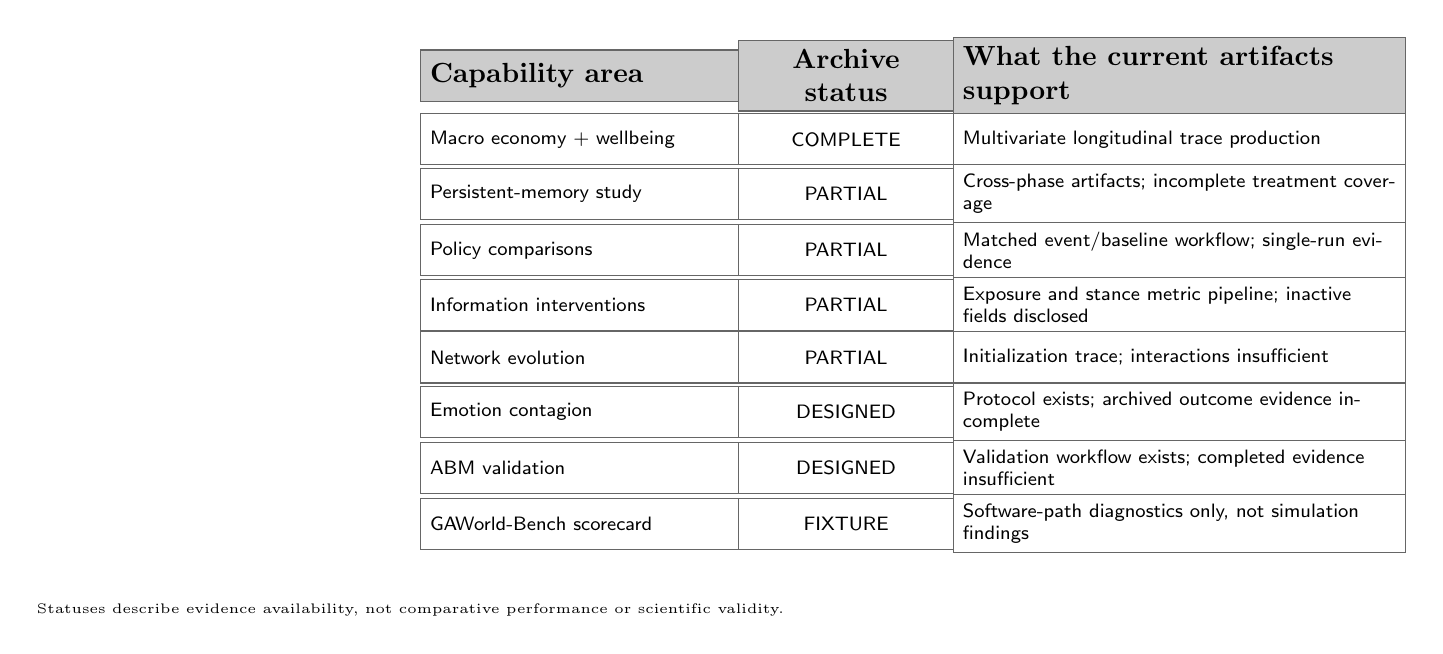
\begin{tikzpicture}[font=\sffamily\scriptsize]
\matrix (m) [matrix of nodes,
 nodes={draw=black!60,minimum height=6.5mm,anchor=center,align=center},
 column 1/.style={nodes={text width=38mm,anchor=west,align=left}},
 column 2/.style={nodes={text width=25mm}},
 column 3/.style={nodes={text width=55mm,anchor=west,align=left}},
 row 1/.style={nodes={fill=black!20,font=\bfseries}},
 row sep=-\pgflinewidth,column sep=-\pgflinewidth] {
 Capability area & Archive status & What the current artifacts support \\
 Macro economy + wellbeing & COMPLETE & Multivariate longitudinal trace production \\
 Persistent-memory study & PARTIAL & Cross-phase artifacts; incomplete treatment coverage \\
 Policy comparisons & PARTIAL & Matched event/baseline workflow; single-run evidence \\
 Information interventions & PARTIAL & Exposure and stance metric pipeline; inactive fields disclosed \\
 Network evolution & PARTIAL & Initialization trace; interactions insufficient \\
 Emotion contagion & DESIGNED & Protocol exists; archived outcome evidence incomplete \\
 ABM validation & DESIGNED & Validation workflow exists; completed evidence insufficient \\
 GAWorld-Bench scorecard & FIXTURE & Software-path diagnostics only, not simulation findings \\
};
\node[font=\tiny,anchor=west,below=4mm of m.south west] {Statuses describe evidence availability, not comparative performance or scientific validity.};
\end{tikzpicture}
\end{document}
